\chapter{Sistemas de numeración}
La información que queremos utilizar en un sistema informático debe estar representada de alguna manera que el ordenador pueda entender.

En sistemas orales, o escritos, lo habitual es hacer uso de un idioma concreto mediante un alfabeto conocido. En informática se hace uso de distintos sistemas de numeración para representar tanto números como el resto de información.

\section{Sistema decimal}
El ser humano, desde hace tiempo ha utilizado como sistema para contar el sistema decimal, representado mediante el sistema \href{https://es.wikipedia.org/wiki/N%C3%BAmeros_ar%C3%A1bigos}{arábigo}. Posiblemente se adoptó este sistema por contar con 10 dedos en las manos.

El sistema numérico decimal está basado en diez símbolos ordenados (0, 1, 2, 3, 4, 5, 6, 7, 8, 9), situados de manera ponderada (cada posición tiene un peso específico), que permiten representar las cantidades deseadas. Debido a que hacemos uso de diez símbolos se dice que utiliza la \textbf{base 10}.

%\subsection*{Representación}
Cuando se combina con otros sistemas de numeración, debemos indicar la base en la forma $ \mathbf{19_{(10}} $ , es decir, poniendo un pequeño “\textbf{(10}” a la derecha del número representado la base 10.

La representación de cualquier combinación del sistema decimal se puede representar en forma de potencia, donde la base es 10 y el exponente es la posición en la que se sitúa el símbolo.

Vamos a tomar como ejemplo el siguiente número: \textbf{146}. La representación en forma de potencias:

\begin{center}
    \vspace{-10pt}
    $ 146 = 100+40+6 $

    $ 146 = 1\times100 + 4\times10 + 6\times1 $

    $ 146 =1\times10^2 + 4\times10^1 + 6\times10^0 $
\end{center}

Como se puede comprobar, lo que hemos hecho ha sido coger cada símbolo representado y lo hemos multiplicado por la base (en este caso base 10) y a la base le hemos puesto el exponente de la posición en la que se encuentra. \textbf{El símbolo de más a la derecha tiene como exponente el cero}, y hacia la izquierda el exponente se incrementa en uno para cada posición.


\hypertarget{binario}{}
\section{Sistema binario}

En informática el sistema binario es el más importante ya que es el sistema que internamente utilizan los circuitos digitales. En este sistema sólo se hace uso de dos símbolos, el “0” y el “1”, y por tanto \textbf{su base es 2}. Los dos dígitos se denominan \textbf{bits} (contracción de \textbf{binary digit}).

%\subsection*{Representación}

Para representar que estamos haciendo uso del sistema binario debemos indicar la base al lado del número, por ejemplo: $\mathbf{ 101001_{(2}} $. Como se puede ver es añadir “\textbf{(2}” en pequeño al final del último símbolo.


\section{Sistema hexadecimal}

Esta vez necesitamos dieciséis símbolos ordenados, así que es un sistema de \textbf{base 16}. Para la representación se hace uso de los símbolos numéricos que conocemos (0, 1, 2, 3, 4, 5, 6, 7, 8, 9) y para representar los siguientes, las letras “A”, “B”, “C”, “D”, “E” y “F”, de esta manera formamos los 16 símbolos que necesitamos.

Teniendo en cuenta esto, podemos hacer la representación directa de que $\mathbf{A_{(16} = 10_{(10}}$ y que $\mathbf{E_{(16} = 14_{(10}}$.

En informática es muy habitual hacer uso del sistema hexadecimal a la hora de trabajar con \textbf{bytes} (que es una “palabra” de \textbf{8 bits}). Un símbolo hexadecimal se representa como 4 bits, por lo que necesitaríamos 2 símbolos hexadecimales para un byte.

También se usa durante la edición de código en formato de datos, o durante la programación en ensamblador.

%\subsection*{Representación}
Al igual que con los sistemas anteriores, debemos añadir la base cuando estemos utilizando el sistema hexadecimal: $\mathbf{ F17A_{(16}} $ , $\mathbf{ FBE1D_{(16}} $ , $\mathbf{ 1FAB27_{(16}} $


\section{Sistema octal}
En ordenadores antiguos era habitual hacer uso del sistema octal. Hoy día se usa más como sistema intermedio entre binario y hexadecimal.

Esta vez nos basamos en ocho símbolos ordenados (0, 1, 2, 3, 4, 5, 6, 7), que, al combinarlos, permiten representar las cantidades deseadas. Debido a que hacemos uso de ocho símbolos se dice que utiliza la \textbf{base 8}.

%\subsection*{Representación}
Para representar la base, debemos añadir “(8” a la derecha del número que hayamos indicado, como por ejemplo: $\mathbf{ 770_{(8} }$ , $\mathbf{ 175_{(8}} $


\section{Conversiones entre los distintos sistemas de numeración}

Hasta ahora no nos habíamos encontrado con distintos sistemas de numeración, pero ahora que conocemos cuatro de ellos, tenemos que saber que existe la posibilidad de realizar conversiones entre ellos.


Una vez entendidos los distintos sistemas de numeración nos tiene que quedar claro que aunque la representación de los símbolos sea la misma, el número o cantidad representada no es la misma. Por ejemplo:

\errorbox{
    \begin{center}
        $\mathbf{ 1010_{(10}  \neq  1010_{(2}  \neq  1010_{(16}  \neq 1010_{(8}} $
    \end{center}
}

A continuación se va a explicar cómo realizar conversiones entre los distintos sistemas de numeración que hemos visto, y a modo de resumen está la \hyperlink{tabla_conversiones_directas}{tabla de conversiones directa}.

\subsection{Conversión de decimal a...}
La manera más sencilla para realizar las distintas conversiones partiendo de un número decimal es hacer divisiones sucesivas usando la base a la que queremos realizar la conversión.

\subsection*{... binario}
Se trata de dividir sucesivamente el número decimal y los sucesivos cocientes entre dos (la base binaria).

Vamos a utilizar como ejemplo el número decimal $\mathbf{27_{(10}}$ :

\begin{center}
    \vspace{-20pt}
    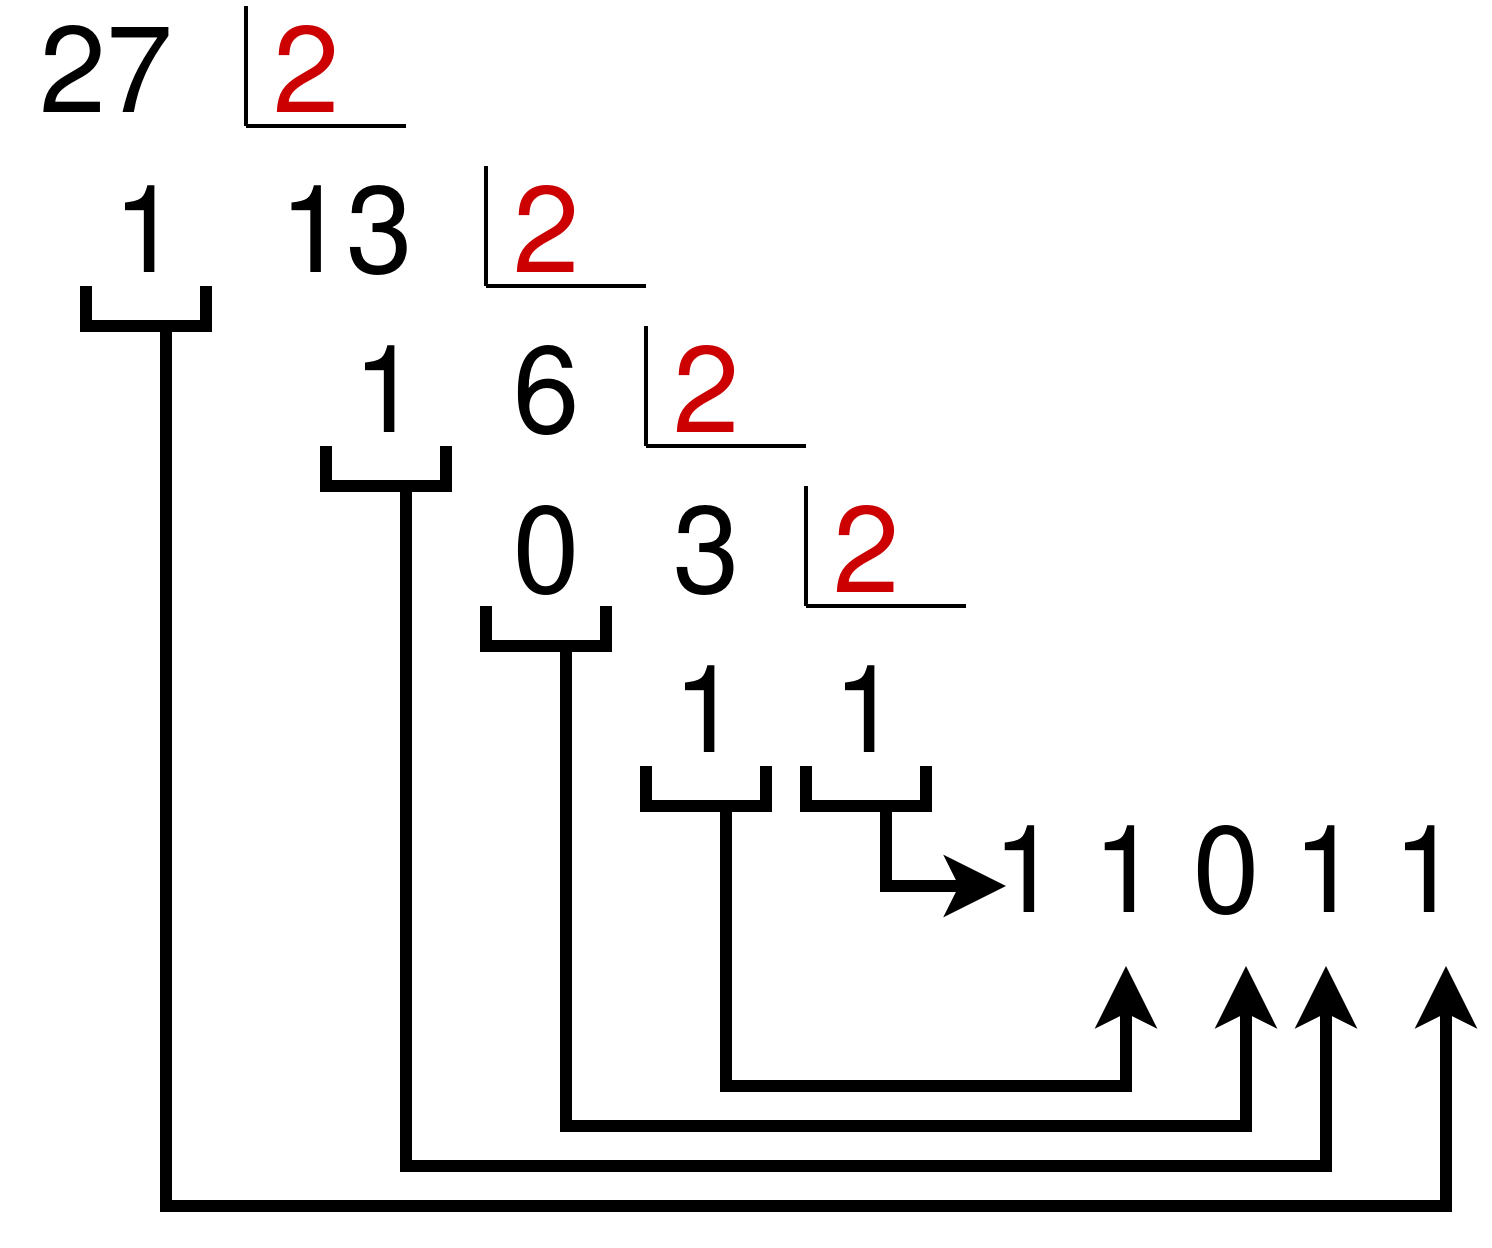
\includegraphics[width=0.29\linewidth]{decimal_binario.png}
    \vspace{-20pt}
\end{center}

\textbf{Los restos los cogemos en orden inverso} para obtener la siguiente equivalencia: $\mathbf{27_{(10} = 11011_{(2}}$

\subsection*{... hexadecimal}
Se trata de dividir sucesivamente el número decimal y los sucesivos cocientes entre 16 (la base hexadecimal). Cuando el cociente o resto sea entre 10 y 15, habrá que cambiarlo por la letra correspondiente.

\begin{center}
    \vspace{-10pt}
    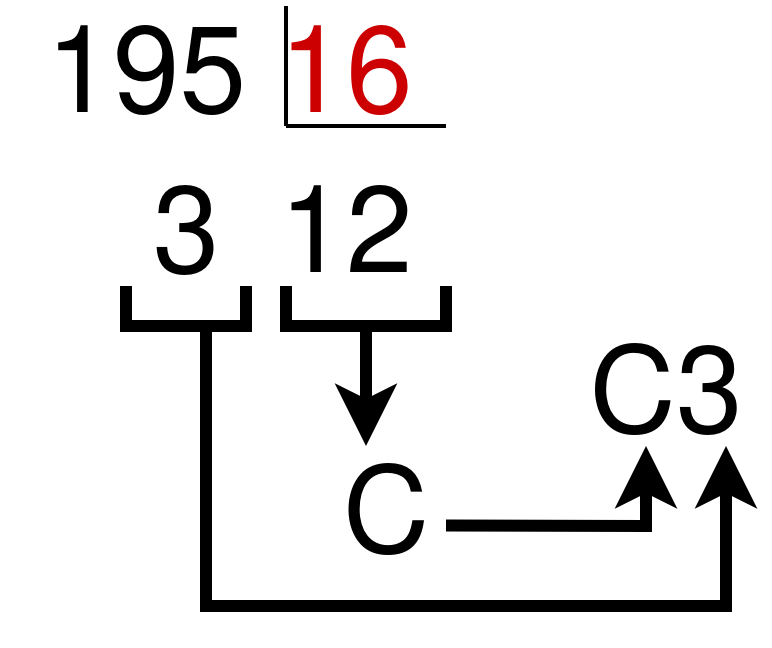
\includegraphics[width=0.2\linewidth]{decimal_hexadecimal.png}
    \vspace{-15pt}
\end{center}

\textbf{Los restos los cogemos en orden inverso} para obtener la siguiente equivalencia: $\mathbf{195_{(10} = C3_{(16}}$

\subsection*{... octal}
Al igual que los anteriores, hacemos divisiones sucesivas:

\begin{center}
    \vspace{-10pt}
    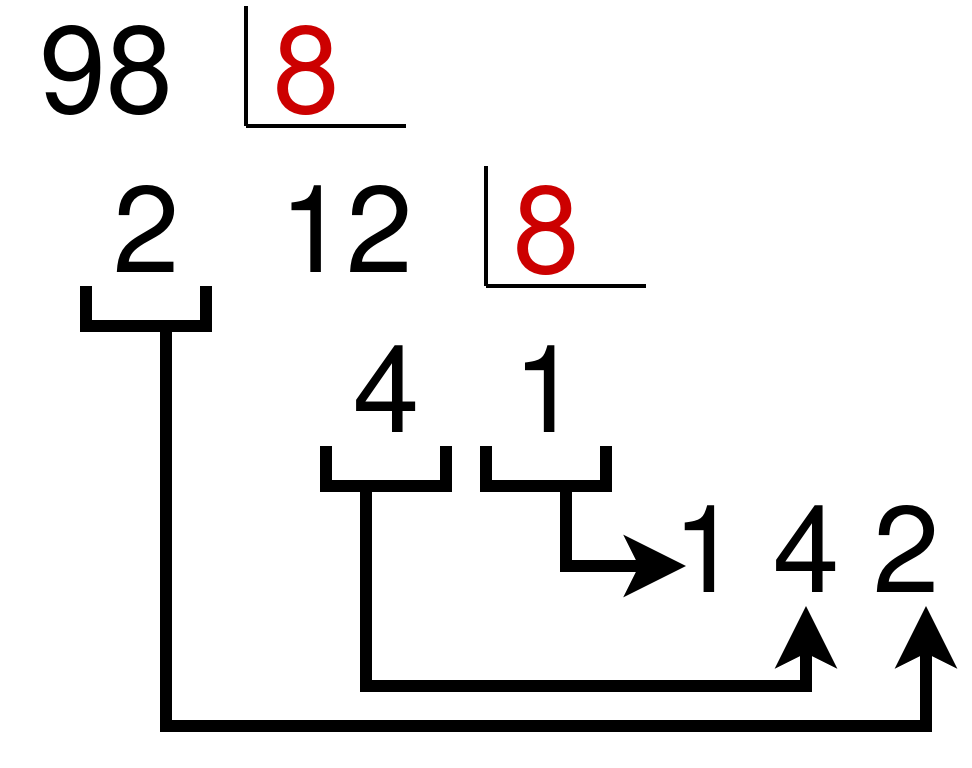
\includegraphics[width=0.25\linewidth]{decimal_octal.png}
    \vspace{-15pt}
\end{center}

\textbf{Los restos los cogemos en orden inverso} para obtener la siguiente equivalencia: $\mathbf{98_{(10} = 142_{(8}}$


\subsection{Conversión de binario a...}

\subsection*{... decimal}
El sistema de numeración binario es un sistema posicional donde cada dígito binario (bit) tiene un valor basado en su posición relativa al \textbf{LSB} (\textit{Least Significant Bit} = bit menos significativo, que es el que está más a la derecha y que tiene el menor valor).

Cualquier número binario puede convertirse a su equivalente decimal multiplicando cada bit por la base (2) y usando como exponente la posición (siendo 0 el exponente del bit de más a la derecha). Para ilustrarlo, cojamos como ejemplo el número binario $\mathbf{11011_{(2}}$:

\begin{center}
    \vspace{-20pt}

    $ \mathbf{11011_{(2}} $

    $ \mathbf{1\times2^4 + 1\times2^3 + 0\times2^2 + 1\times2^1 + 1\times2^0} $

    $ \mathbf{16 + 8 + 0 + 2 + 1 = 27_{(10}} $
    \vspace{-15pt}
\end{center}

Nótese que el procedimiento consiste en determinar los valores (es decir, las potencias de 2) de cada posición de bit que contenga un 1 y luego sumarlos.

Nótese también que el \textbf{MSB} (\textit{Most Significant Bit} = bit más significativo,\textbf{ el que está más a la izquierda}, el que tiene mayor valor) tiene un valor de $\mathbf{2^4}$ a pesar de que es el quinto bit. Esto se debe a que el \textbf{LSB} (\textit{Least Significant Bit}, el bit menos significativo, el que está a la derecha) es el primer bit y tiene un valor de $\mathbf{2^0}$.

\subsection*{... octal}
Para convertir un número binario a octal \textbf{se agrupan los dígitos de 3 en 3 empezando desde el lado derecho} hacia la izquierda, sustituyendo cada trío de dígitos binarios por su equivalente en octal.

Si en el lado izquierdo quedase algún bit “suelto” (sin formar un grupo de 3), se pueden poner “0” a la izquierda.

Cogemos como ejemplo el número binario $\mathbf{1100101001001_{(2}}$ para pasarlo a octal, haremos:

\begin{center}
    \vspace{-15pt}
    $\mathbf{001\ \ 100\ \ 101\ \ 001\ \ 001_{(2} = 14511_{(8}}$
    \vspace{-15pt}
\end{center}

\subsection*{... hexadecimal}
Similar al caso anterior, pero en este caso \textbf{la agrupación que se realiza debe de ser de 4 en 4 bits}. Si usamos el mismo ejemplo anterior $\mathbf{1100101001001_{(2}}$ :

\begin{center}
    \vspace{-15pt}
    $\mathbf{0001\ \ 1001\ \ 0100\ \ 1001_{(2} = 1949_{(16}}$
    \vspace{25pt}
\end{center}



\subsection{Conversión de hexadecimal a...}
\subsection*{... binario}
Para pasar de hexadecimal a binario convertiremos cada símbolo hexadecimal a 4 dígitos binarios.

\begin{center}
    \vspace{-15pt}
    $\mathbf{F17A_{(16} = 1111\ \ 0001\ \ 0111\ \ 1010_{(2}}$

    $\mathbf{1A4F_{(16} = 0001\ \ 1010\ \ 0100\ \ 111_{(2}}$
    \vspace{-15pt}
\end{center}


\subsection*{... decimal}
Al igual que hemos hecho con las conversiones previas a decimal, se podría realizar haciendo potencias de 16, pero se entiende que es más complicado de realizar.

Por lo tanto, \textbf{la manera más sencilla es pasar primero a binario} como acabamos de ver \textbf{y posteriormente convertir ese binario a decimal} como hemos visto previamente.

\subsection*{... octal}
Pasar primero a binario y después a octal.



\subsection{Conversión de octal a...}
\subsection*{... binario}
Cada dígito en octal se convierte en su representación en 3 bits:

\begin{center}
    \vspace{-15pt}
    $\mathbf{167_{(8} = 001\ \ 110\ \ 111_{(2}}$

    $\mathbf{253_{(8} = 010\ \ 101\ \ 011_{(2}}$
    \vspace{-15pt}
\end{center}
Los ceros de la izquierda se podrían quitar, ya que no alteran el valor.

\subsection*{... decimal}
Se puede realizar de dos maneras. La primera es hacer uso de potencias de 8 (similar al paso de pasar de binario a decimal, pero cambiando la base):

\begin{center}
    \vspace{-15pt}
    $\mathbf{157_{(8} = 1\times8^2 + 5\times8^1 + 7\times8^0 = }$

    $\mathbf{1\times64 + 5\times8 + 7\times1 = }$

    $\mathbf{64 + 40 + 7 = 111_{(10}}$

    Resultado: $\mathbf{157_{(8} = 111_{(10}}$
    \vspace{-15pt}
\end{center}

Con números grandes puede ser un poco complicado calcular las potencias de 8, por lo que \textbf{la alternativa es pasarlo primero a binario} como hemos visto, \textbf{y después pasarlo de binario a decimal}.

\subsection*{... hexadecimal}
La manera más sencilla es realizar la conversión primero a binario tal como hemos visto, y posteriormente pasar el número binario a hexadecimal como se ha visto previamente.